\documentclass[10pt]{article}
\usepackage{graphicx}
\usepackage{subcaption}
\usepackage[T1]{fontenc}
\usepackage{amsmath}
\usepackage{lipsum}
\usepackage{amsfonts}
\usepackage{hyperref}
\usepackage[utf8]{inputenc}
\usepackage[letterpaper,margin=1in]{geometry}
\usepackage[parfill]{parskip}
\usepackage[europeanresistors, american]{circuitikz}
\usetikzlibrary{arrows,shapes,calc,positioning}
\usetikzlibrary{shapes}
\usetikzlibrary{plotmarks}
\usepackage{tikz}
\usepackage{pgfplots}
\usepackage{xparse}
\usetikzlibrary{decorations.markings,positioning}
\definecolor{whitesmoke}{rgb}{0.90, 0.90, 0.90}
\definecolor{lightgray}{rgb}{0.73, 0.73, 0.73}% overrides default?
\definecolor{dimgray}{rgb}{0.51, 0.51, 0.51}
\pgfplotsset{compat=newest}
\usepgfplotslibrary{units}
\newcommand{\oscope}[2] % #1 = name , #2 = rotation angle
{
    \draw[thick,rotate=#2] (#1) circle (12pt)
    (#1) ++(-0.35,-0.1) -- ++(0.3,0.3) --++(0,-0.3)-- ++(0.3,0.3) --++(0,-0.3);
}
\def\therefore{\boldsymbol{\text{ }
\leavevmode
\lower0.4ex\hbox{$\cdot$}
\kern-.5em\raise0.7ex\hbox{$\cdot$}
\kern-0.55em\lower0.4ex\hbox{$\cdot$}
\thinspace\text{ }}}
\pgfarrowsdeclarecombine{dimarrow}{dimarrow}{latex}{latex}{}{}
\NewDocumentCommand\Dimline { m m o } {
  \draw[|-|, thick, shorten >=-.5\pgflinewidth, shorten <=-.5\pgflinewidth,
  decoration={markings, % switch on markings
    mark=at position 0 with {\arrowreversed[scale=0.5]{dimarrow}};,
    mark=at position .5 with {\IfValueT{#3}{\node [black, fill=white] {#3};}},
    mark=at position 1 with {\arrow[scale=0.5]{dimarrow}};,
  },
  postaction=decorate] #1 -- #2 ;
}
\pgfplotstableread{
x   SC   UNKWN
0   -70.430 -53.823
5   -56.743 -53.384
10  -51.003 -52.223
15  -47.270 -50.688  
20  -43.939 -49.049
25  -43.110 -47.984
30  -42.755 -47.163
35  -42.707 -46.770
40  -42.797 -46.310
45  -43.461 -46.294
50  -44.326 -46.392
55  -46.781 -46.920
60  -47.946 -47.690
65  -51.511 -48.500
70  -57.215 -49.421
75  -70.787 -50.184
80  -60.603 -49.948
}\wavform

\vspace{-8ex}
\date{}
\begin{document}

\title{\textbf{\Large{\textsc{ECE320:} Fields and Waves}} \\ \Large{Lab 2 Report: Standing Waves and Waveguides} \\ \textbf{\small{PRA106}}\vspace{-0.3cm}}
\author{Alp Tarım, Pranshu Malik \\ \footnotesize{1003860128}, \footnotesize{1004138916}}

\maketitle

\section{Introduction}
\vspace{-0.3cm}

This laboratory session was focused on investigating the voltage standing wave (VSW) pattern along a microstrip transmission line, 
as well as its depedance on the load impedance. Figure 1 shows the diagram of a microstrip line that sits on the PCB substrate at the bottom and free
space (or air) above, due to which the voltage wave effectively travels through $\epsilon_\text{eff}\epsilon_0$. We measure the fringing electric field 
using a probe, acting as a monopole antenna, at the top of the strip. Since the measured, vertically oriented, electric field is proportional to 
the voltage at that position we are able to determine the VSW pattern along the line.
\begin{figure}[h]
  \centering
  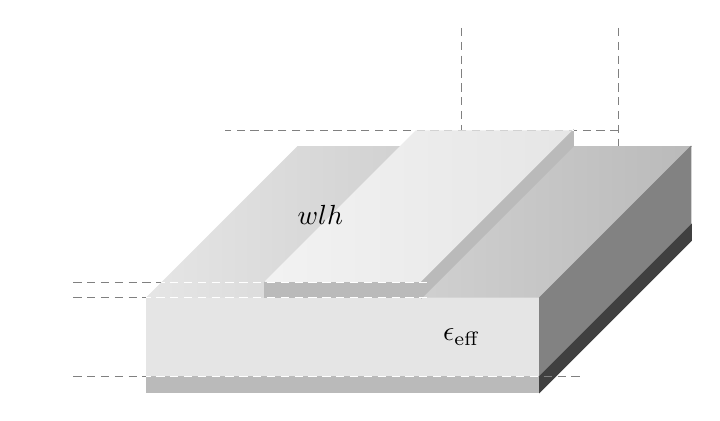
\begin{tikzpicture}
    \draw [lightgray] (0,1,0) coordinate (bl) -- (5,1,0) coordinate (br);
    \filldraw [whitesmoke] (0,0,5) coordinate (fll) -- (0,1,5) coordinate (ftl) -- (5,1,5) coordinate (ftr) -- (5,0,5) coordinate (flr) -- cycle;
    \shade [left color = whitesmoke, right color = lightgray] (bl) -- (br) -- (ftr) -- (ftl) -- cycle;
    \filldraw [dimgray] (5,0,0) coordinate (blr) -- (flr) -- (ftr) -- (br);
    \filldraw [lightgray] (fll) rectangle (5,-0.2,5) coordinate (flr2);
    \filldraw [darkgray] (flr2) -- (5,-0.2,0) coordinate (blr2) -- (blr) -- (flr) -- cycle;
    \filldraw [lightgray] (1.5,1.2,5) coordinate (ftl-1) -- (3.5,1.2,5) coordinate (ftr-1) -- (3.5,1,5) coordinate (flr-1) -- (1.5,1,5) coordinate (fll-1) -- cycle;
    \shade [left color = whitesmoke!50, right color = whitesmoke] (1.5,1.2,0) coordinate (btl-1) -- (3.5,1.2,0) coordinate (btr-1) -- (ftr-1) -- (ftl-1) -- cycle;
    \filldraw [lightgray] (flr-1) -- (ftr-1) -- (btr-1) --  (br -| btr-1) -- cycle;
    \node at (4,0.5,5) {$\epsilon_\text{eff}$};
    \coordinate (nA1) at (1.5,2.5,0);
    \coordinate (nB1) at (3.5,2.5,0);
    \coordinate (nA2) at (-1.5,1.2,0);
    \coordinate (nB2) at (-1.5,1.2,5);
    \coordinate (nA3) at (3,1,5);
    \coordinate (nB3) at (3,1.2,5);
    \coordinate (nA4) at (-1.5,1,5);
    \coordinate (nB4) at (-1.5,0,5);
    \Dimline{(nA1)}{(nB1)}[$w$];
    \Dimline{(nA2)}{(nB2)}[$l$];
    \Dimline{(nA4)}{(nB4)}[$h$];
    \draw [densely dashed, help lines, blend mode=color dodge]  (nB4) -- (flr) (btr-1) -- (nA2)  (nB2) -- (nB3)  (nA4) -- (nA3) (nA1) -- (btl-1) (nB1) -- (btr-1 |- br);
  \end{tikzpicture}
  \caption{A microstrip transmission line\vspace{-1cm}}
\end{figure}

\section{Measurement of Microstrip Line Characteristics}
\vspace{-0.3cm}
We know that since the wave travels in a compound medium -- the PCB substrate and the air -- we will have 
to consider an effective dielectric constant dependant on the geometry as well as the substrate parameters. It has been
found that this is best described using a combination of conformal mapping and empiral formulae, which are:
\[
    \epsilon_{\text{eff}} = \frac{\epsilon_r+1}{2}+\left(\frac{\epsilon_r-1}{2}\right)\left(1+\frac{10}{s}\right)^{-xy}
\]
where $s = \frac{w}{h}$ and
\begin{align*}
    x &= 0.56\left(\frac{\epsilon_r-0.9}{\epsilon_r+3}\right)^{0.05}\\
    y &= 1 + 0.02\ln{\left(\frac{s^4+3.7\cdot10^{-4}s^2}{s^4 + 0.43}\right)} + 0.05\ln{\left(1 + 1.7\cdot10^{-4}s^3\right)}
\end{align*}

The characteristic impedance of a microstrip line can also be found using empiral formulae, such as:

\begin{align*}
    Z_0 &= \frac{60}{\sqrt{\epsilon_{\text{eff}}}}\ln{\left(\frac{6 + (2\pi - 6)e^{-t}}{s} + \sqrt{1 + \frac{4}{s^2}}\right)} \quad \text{where} \quad t = \left(\frac{30.65}{s}\right)^{0.75}
\end{align*}

We measured the width of the microstrip line and used the above formulae to calculate the theoretical values of the
characteristic impedance, effective dielectric constant, the phase velocity of the voltage wave, its wavelength at $f = 1 \text{ GHz}$, 
the reflection coefficient at the short circuit load, and the voltage standing wave ratio (VSWR). The results can be found below in table 1.

\begin{table}[h]
  \[
      \begin{array}{c|c}
          \textbf{Parameter} & \textbf{Value} \\ \hline
          w & 0.3 \text{ cm}\\
          Z_0 & 48.697\Omega\\
          \epsilon_\text{eff} & 3.347\\
          v_p & 1.639\cdot10^8\text{ m}/\text{s}\\
          \lambda & 0.163 \text{ m}\\
          \Gamma_L & -1\\
          \text{VSWR} & \infty
      \end{array}
  \]
  \caption{Theoretically calculated parameters of the microstrip transmission line\vspace{-0.2cm}}
\end{table}

Using the vector network analyzer (VNA) in the lab, we sampled the magnitude of the electric field every 5 mm, starting at 
the location of the first minimum magnitude $d_\text{min}$. The experimental SWR pattern can be found in figure 2.

\begin{figure}[ht]
  \centering
  \resizebox{0.55\textwidth}{!}{
    \begin{tikzpicture}
      \begin{axis}[
          width=\linewidth, % Scale the plot to \linewidth
          grid=major, 
          grid style={dashed,gray!30},
          xlabel={Distance from first minimum, $d_{\text{min}}$, in mm},
          ylabel=Electric field strength in dB,
          legend style={at={(0.8,0.95)},anchor=north},
          x tick label style={rotate=90,anchor=east}
        ]
        \addplot +[black,mark options={fill=black}]
        table[x=x,y=SC,col sep=tab] {\wavform}; 
        \legend{log-mag for short circuit load}
      \end{axis}
    \end{tikzpicture}
  }
  \caption{VSW pattern for a shorted load on the microstrip line\vspace{-0.2cm}}
  \label{VNA_log_mag_shorted}
\end{figure}

Using the data in figure 2, we know that
\[||\tilde V_\text{max}|| = k\cdot ||\tilde E_\text{max}|| = k\cdot 10^{-\frac{42.707}{20}} = k\cdot 0.00732\]
Similarly,
  \[ || \tilde V_\text{min}|| = k\cdot 10^{-\frac{70.430}{20}} = k\cdot 0.00030\]
Thus,
  \[\text{VSWR} := \frac{||\tilde V_\text{max}||}{||\tilde V_\text{max}||} = 24.330\]

Although here the VSWR is large, it is still very small compared to the theoretical value of $\infty$. But to
show that our measurements are still accurate, we can show that the corresponding value of reflection coefficient
at the load, $||\Gamma_L|| = \frac{\text{VSWR}-1}{\text{VSWR}+1} = 0.921 \approx 1$ is close to the theoretical value of 1. We also measured that two consecutive voltage minimums were $\approx 8 \text{ cm}$ apart, thus giving us the wavelength 
of the voltage wave $\frac{\lambda}{2} = 8\text{ cm} \implies \lambda = 16\text{ cm} \approx 16.3\text{ cm}$, since the wavelength 
observed in the SWR pattern is half of the wave's wavelength. Using the above result for wavelength and the chosen frequency of 1 GHz, we get 
$v_p = 1.6\cdot10^8 \text{ m/s} = \frac{c}{\sqrt{\epsilon_\text{eff}}} \implies \epsilon_\text{eff} = 3.511 \approx 3.347$. 
Thus, our measurements do closely match the theoretical results for all the parameters.
\vspace{-0.3cm}

\section{Using Standing Wave Patterns for Load Calculations}

\vspace{-0.2cm}
Using data from figure 3 and performing similar calculations as above we get
\begin{align*}
  || \tilde V_\text{max}|| = k\cdot 10^{-\frac{46.294}{20}} = k\cdot 0.00484 \quad &\text{and} \quad || \tilde V_\text{min}|| = k\cdot 10^{-\frac{53.823}{20}} = k\cdot 0.00203\\
  \therefore \text{ VSWR} = 2.379 \quad &\text{and} \quad ||\Gamma_L|| = 0.408 
\end{align*}

Here we note that $\Gamma_L = ||\Gamma_L||e^{j\phi_\Gamma}$. To get phase of the reflection coefficient, $\phi_\Gamma$, we recorded the distance of the first minimum from the load towards the 
generator, $d_\text{min} = 6.9 \text{ cm}$, and used previous measurement of $\lambda = 16\text{ cm}$. Thus,
\begin{align*}
  \phi_\Gamma = \pi + \frac{4\pi d_\text{min}}{\lambda}= 8.561\text{ radians}
\end{align*}
We can get the load impedance using our measurements by 
\[
  \Gamma_L  = 0.408e^{j8.561} = \frac{Z_L - Z_0}{Z_L + Z_0} \implies Z_L = 24.568 + j18.2892 \quad [\Omega]
\]

\begin{figure}[hb]
  \centering
  \resizebox{0.55\textwidth}{!}{
    \begin{tikzpicture}
      \begin{axis}[
          width=\linewidth, % Scale the plot to \linewidth
          grid=major, 
          grid style={dashed,gray!30},
          xlabel={Distance from first minimum, $d_{\text{min}}$, in mm},
          ylabel=Electric field strength in dB,
          legend style={at={(0.8,0.95)},anchor=north},
          x tick label style={rotate=90,anchor=east}
        ]
        \addplot +[black,mark options={fill=black}]
        table[x=x,y=UNKWN,col sep=tab] {\wavform}; 
        \legend{log-mag for unknown load}
      \end{axis}
    \end{tikzpicture}
  }
  \caption{VSW pattern for the unknown load on the microstrip line}
  \label{VNA_log_mag_unknown}
\end{figure}

This impedance was also measured directly using the VNA on a Smith chart, shown in figure 4. The direct measurement yielded
$Z_\text{L,VNA} = 29.974 + j4.581$, which has magnitude $||Z_\text{L,VNA}|| = 30.322$ which is very close to the magnitude of our 
derived impedance $||Z_L|| = 30.628$. Since the expression for load impedance, $Z_L$, is dependant on both $\phi_\Gamma$ and $||\Gamma||$, slight 
errors in measurement make a large difference to the final result due to error multiplication. Our measurements have still 
given us a good estimate of the actual impedance, and this is also shown on the Smith chart in figure 5.

\begin{figure}[ht]
  \centering
  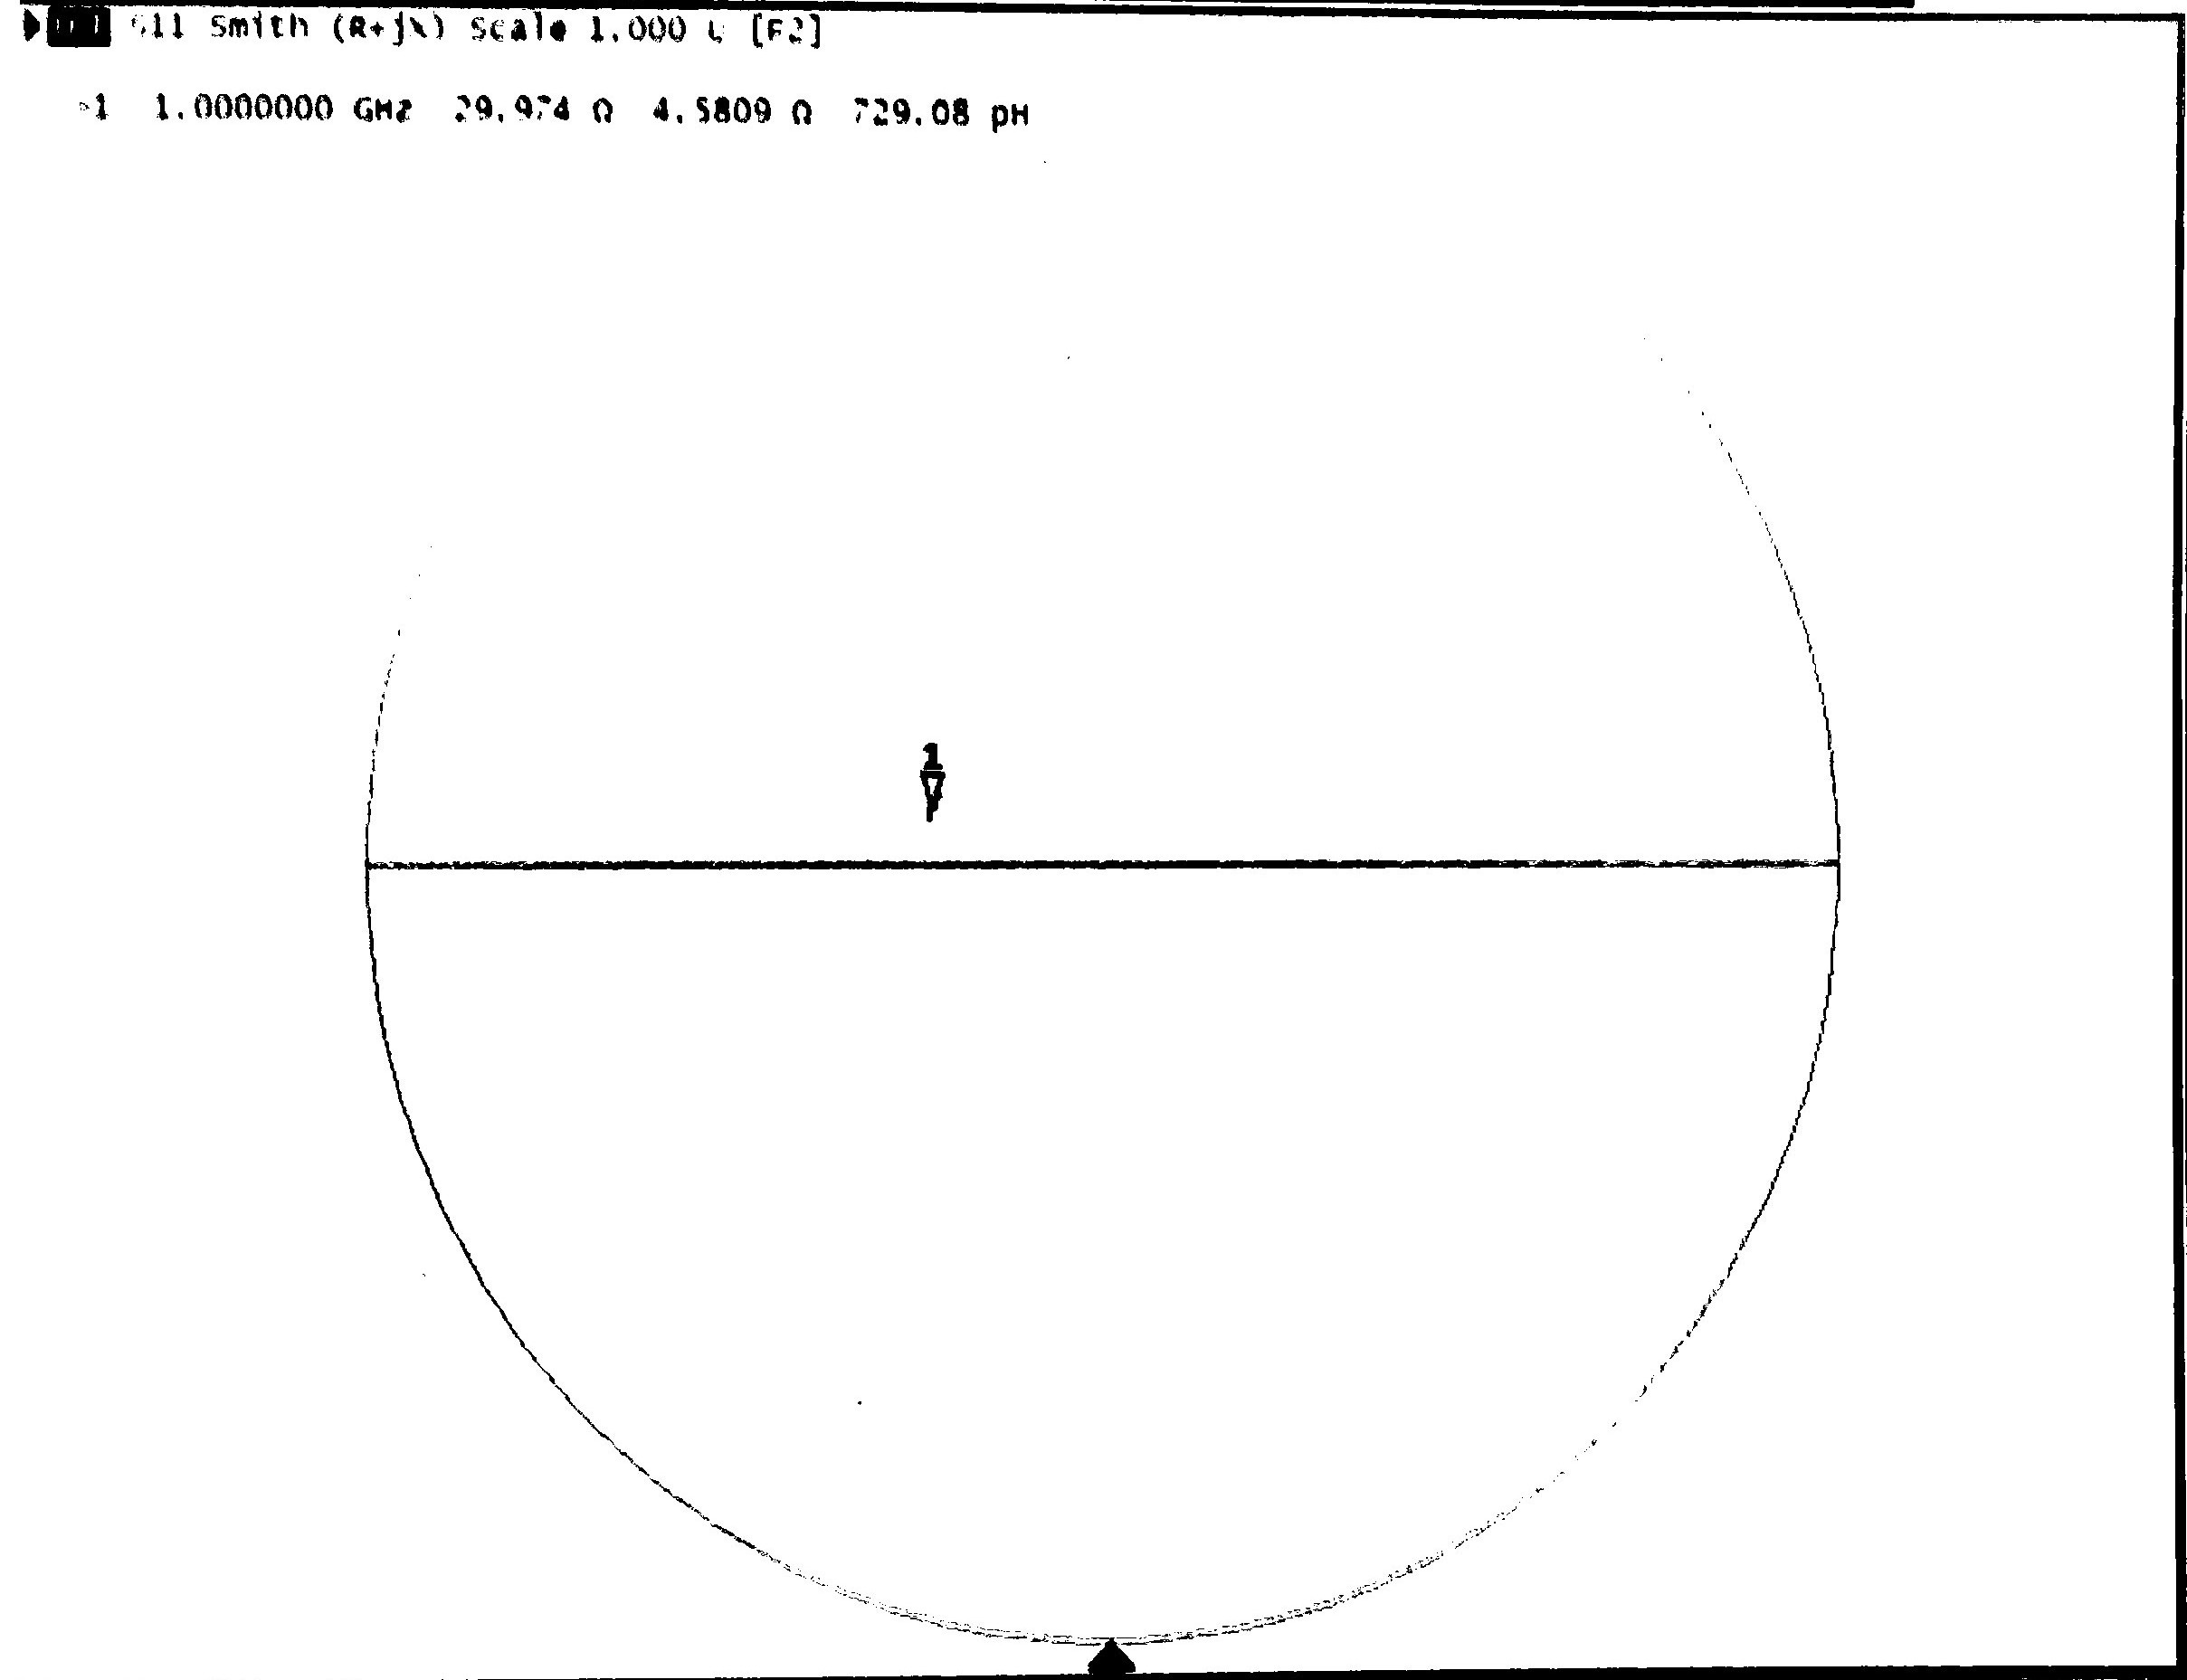
\includegraphics[width=0.45\textwidth]{../photos/lab2/unkwn-load.jpg}
  \caption{Impedance of the unkown load measured by the VNA\vspace{-0.2cm}}
  \label{tline_matching_z_0}
\end{figure}

We suspect that the error mainly originates from the adapter as well as the load connector since there was a difference in geometry and material (and hence impedance); 
the conector and adapater were coaxial instead of a microstrip structure. Furthermore, there could also be error in accurately measuring the added length of the 
connector.

\begin{figure}[ht]
  \centering
  % 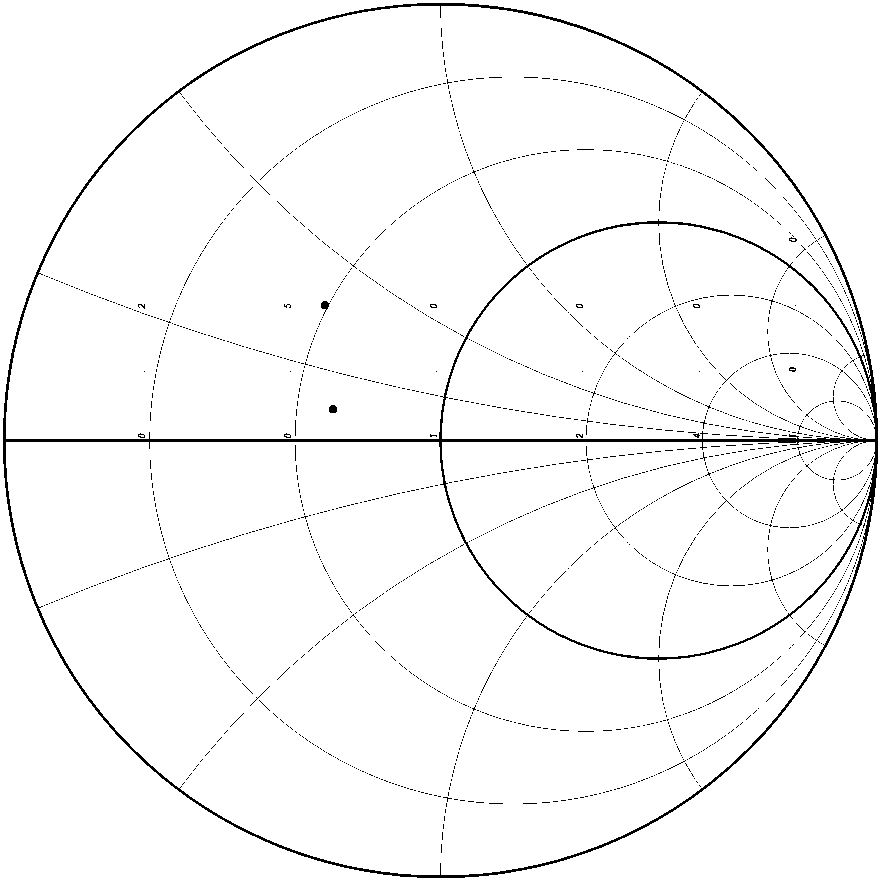
\includegraphics[width=0.6\textwidth]{../photos/lab2/smith-chart.png}
  \begin{tikzpicture}
    \node[inner sep=0pt] (smith) at (0,0)
    {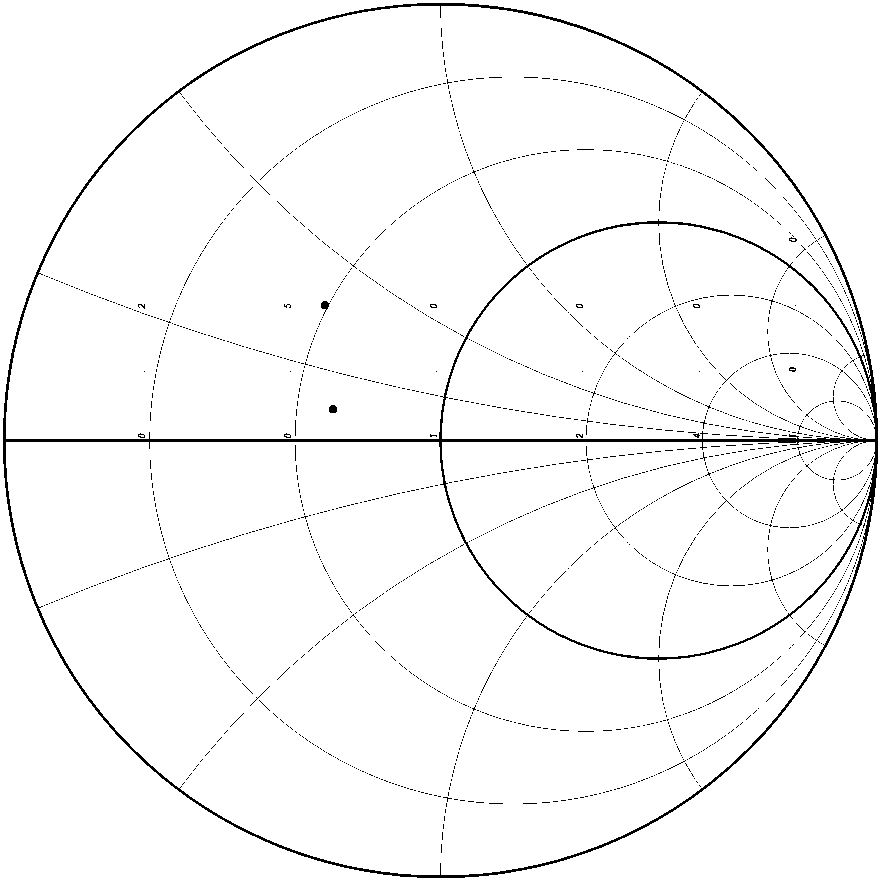
\includegraphics[width=0.6\textwidth]{../photos/lab2/smith-chart.png}};
    \node[draw] at (-2.4,2) {$Z_L = 24.568 + j18.2892$};
    \node[draw] at (-3.5,0.45) {$Z_\text{L,VNA} = 29.974 + j4.581$};
  \end{tikzpicture}
  \caption{Comparison of indirectly and directly measured imepedance on the Smith chart}
\end{figure}

\section{Appendix}

Some key measurements from the log-mag plots on the VNA are shown in figure 6.

\begin{figure}[ht]
  \centering
  \begin{subfigure}[b]{0.45\textwidth}
      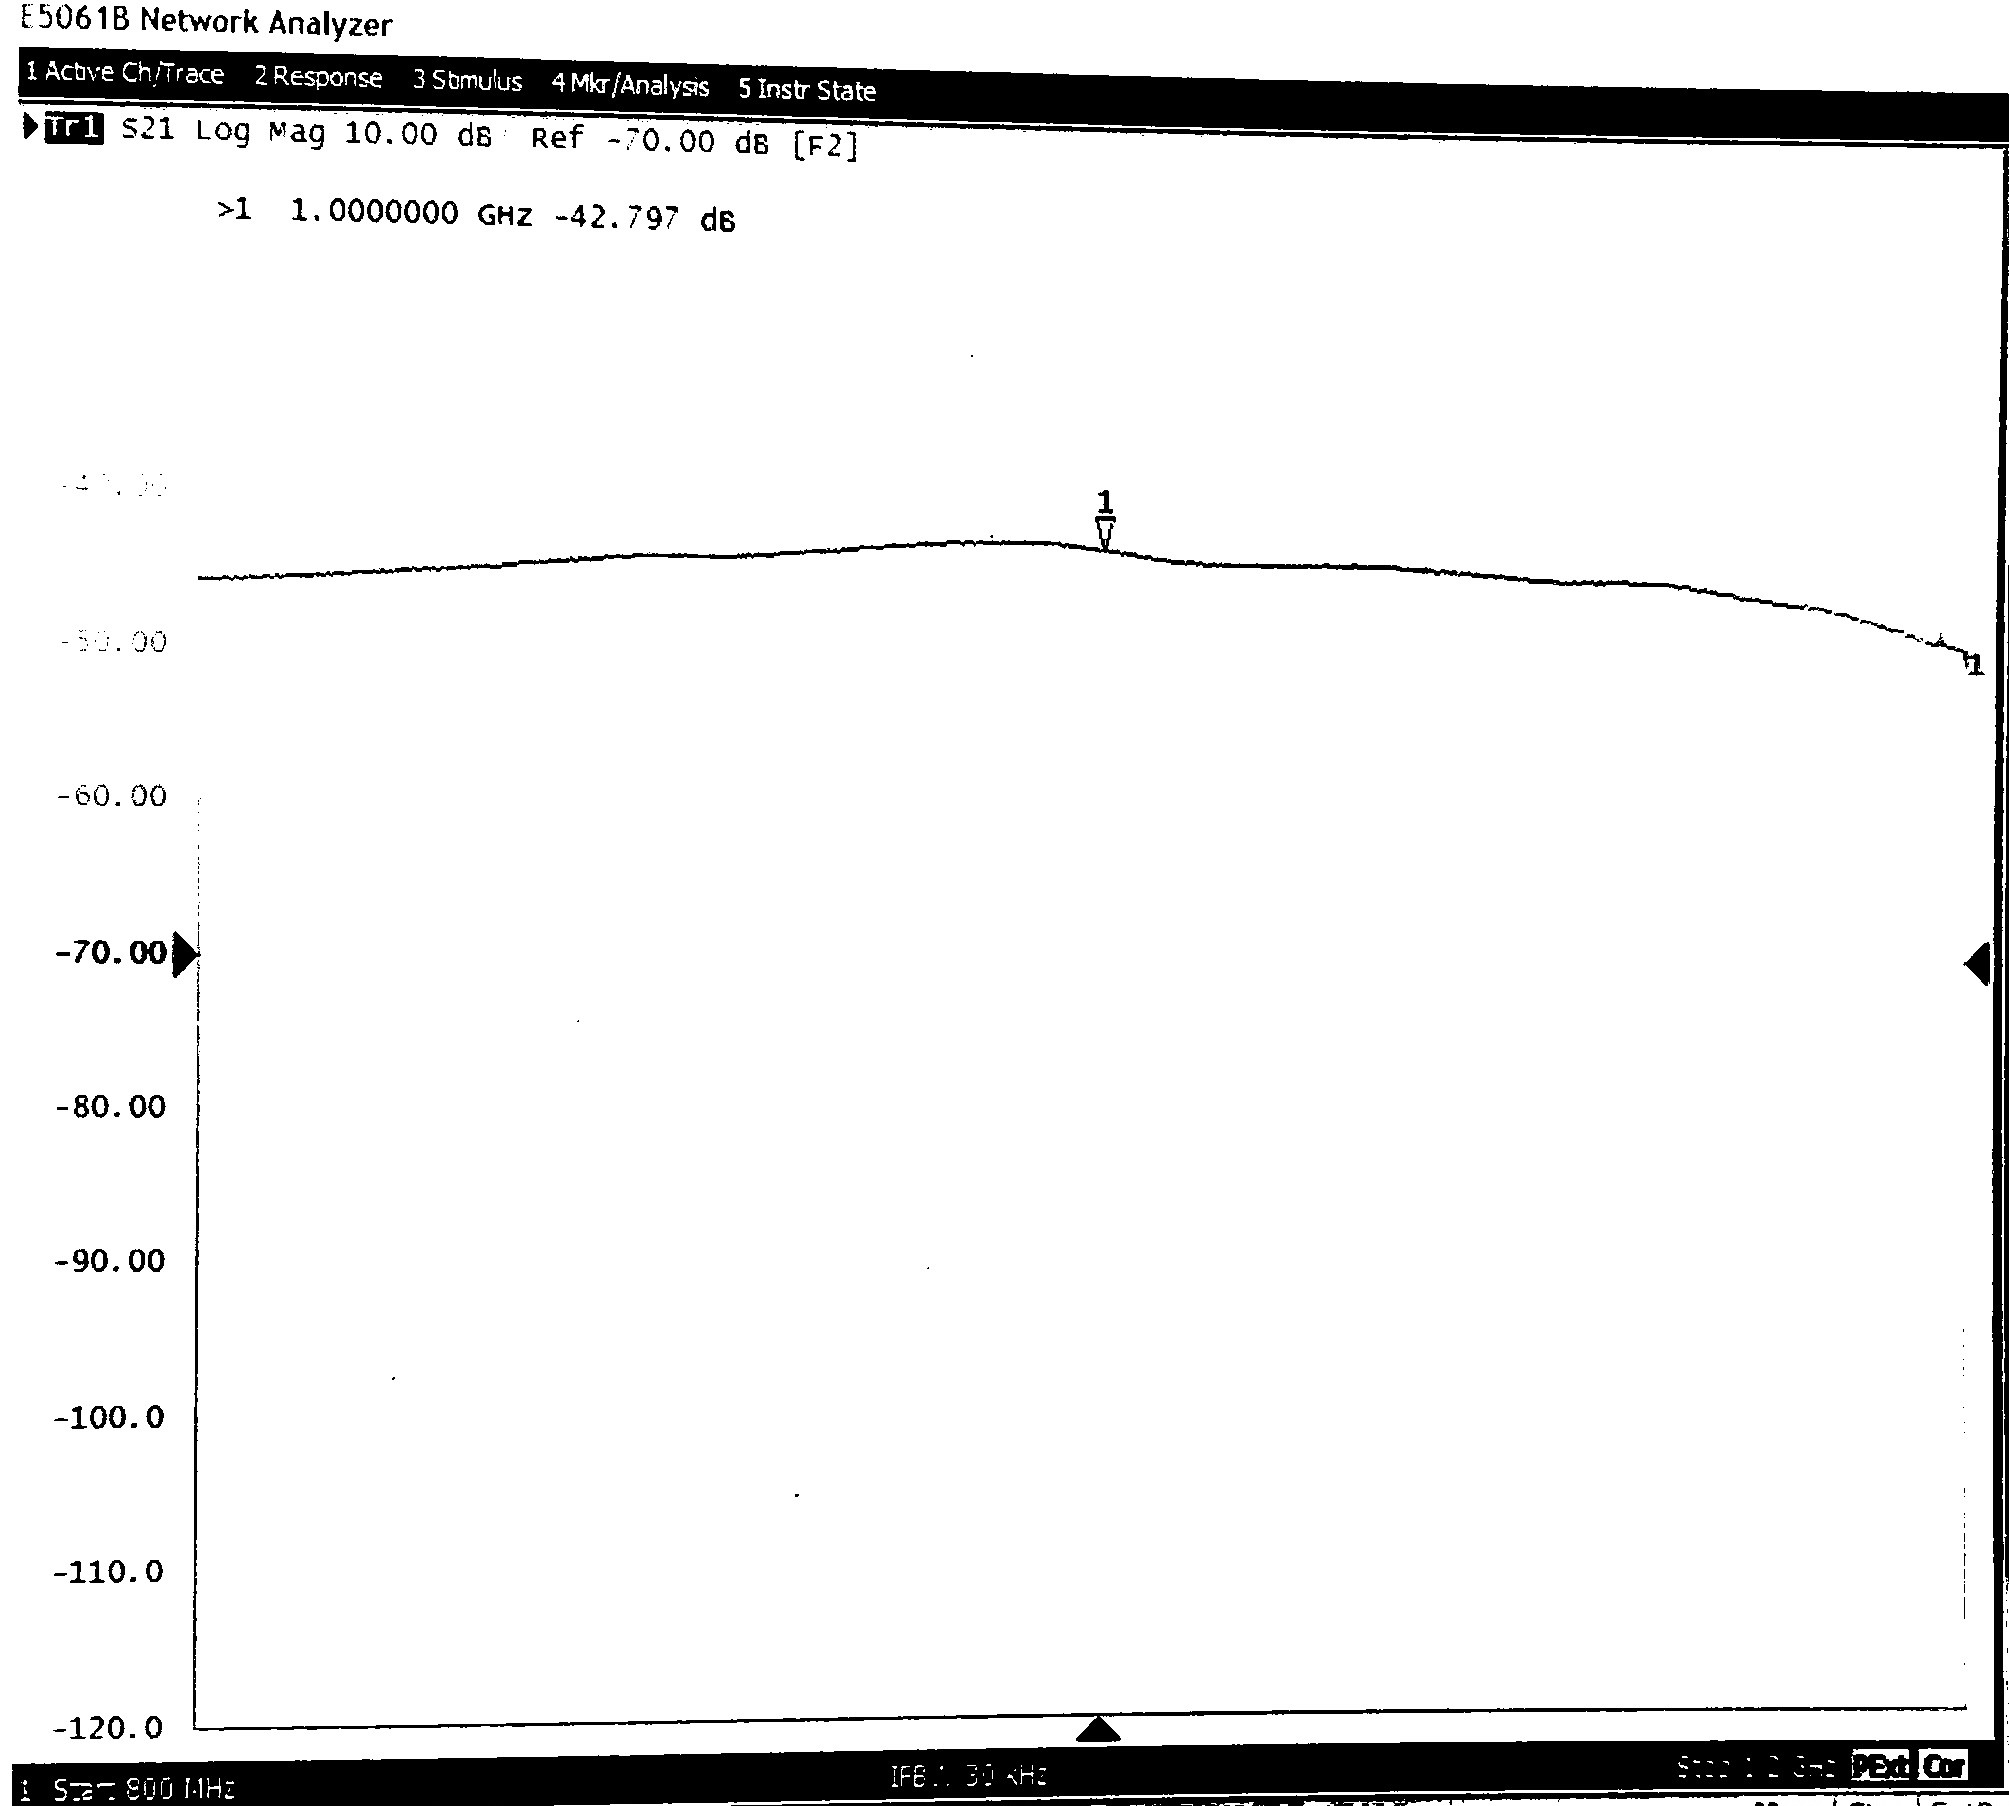
\includegraphics[width=\textwidth]{../photos/lab2/short-cir-peak.jpg}
      \caption{Short circuit load maximum}
  \end{subfigure}
  \quad
  \begin{subfigure}[b]{0.45\textwidth}
      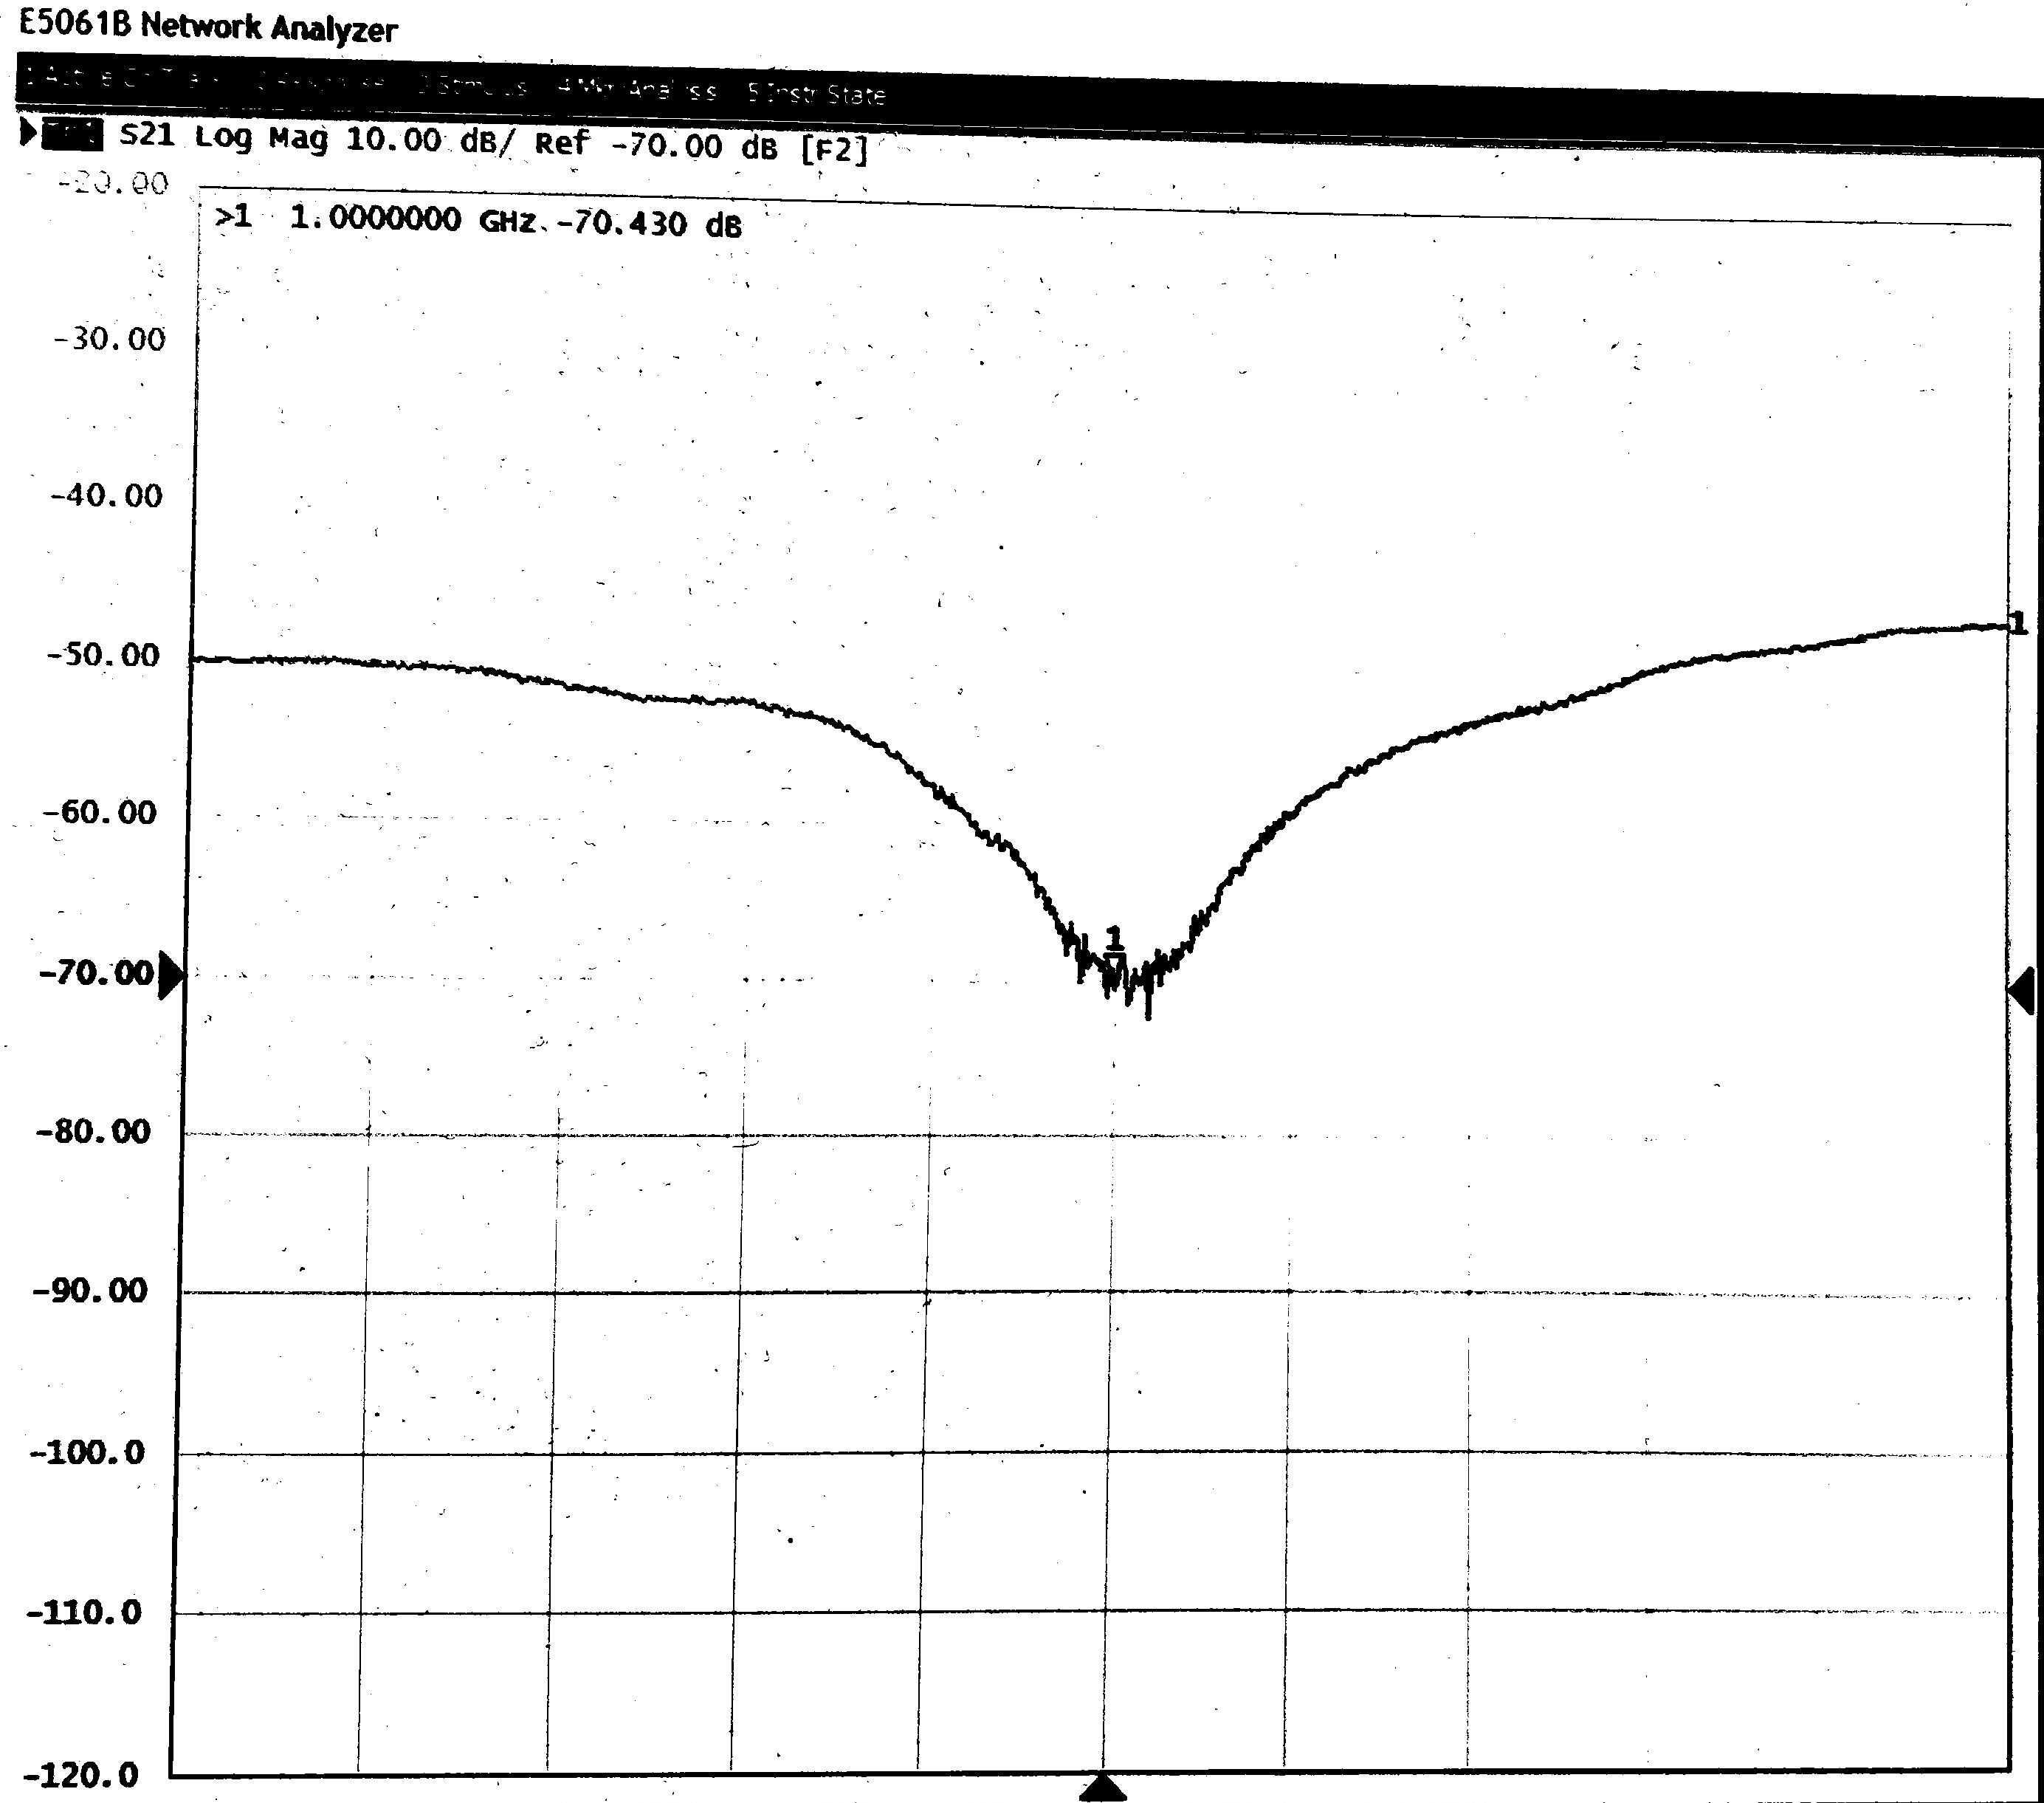
\includegraphics[width=\textwidth]{../photos/lab2/short-cir-valley.jpg}
      \caption{Short circuit load minimum}
  \end{subfigure}
  \begin{subfigure}[b]{0.45\textwidth}
      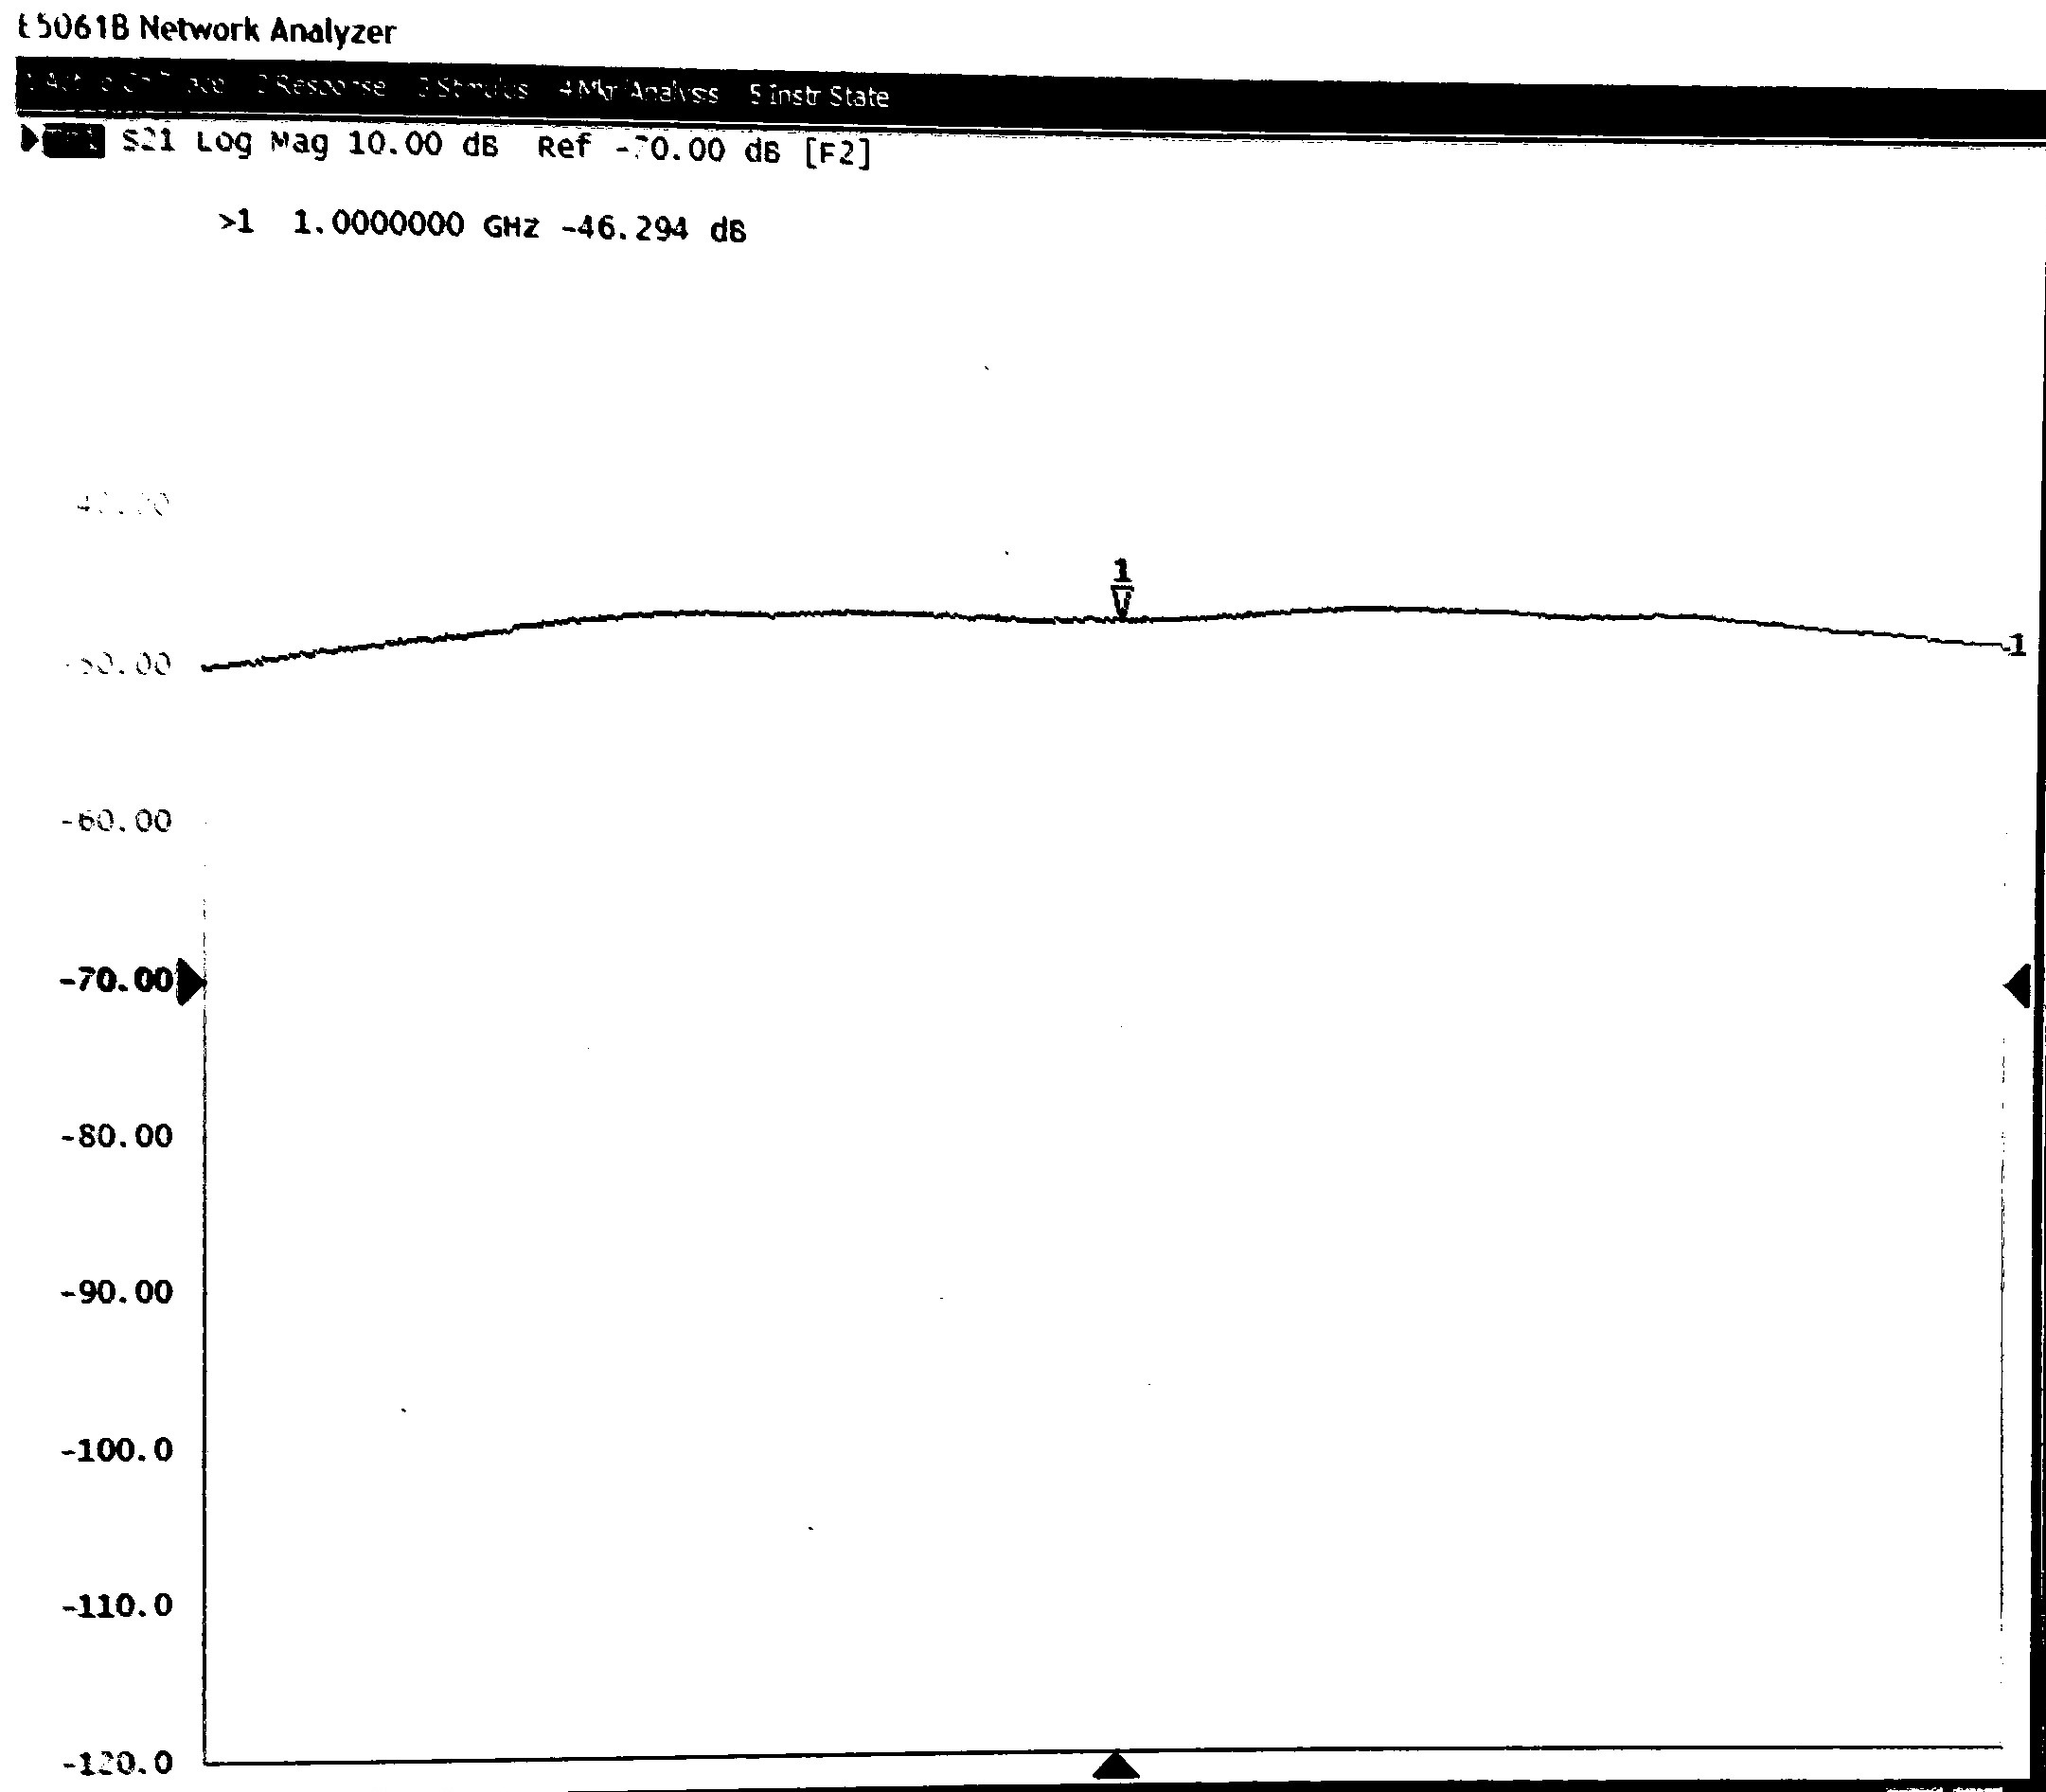
\includegraphics[width=\textwidth]{../photos/lab2/unkwn-load-peak.jpg}
      \caption{Unknown load maximum}
  \end{subfigure}
  \quad
  \begin{subfigure}[b]{0.45\textwidth}
      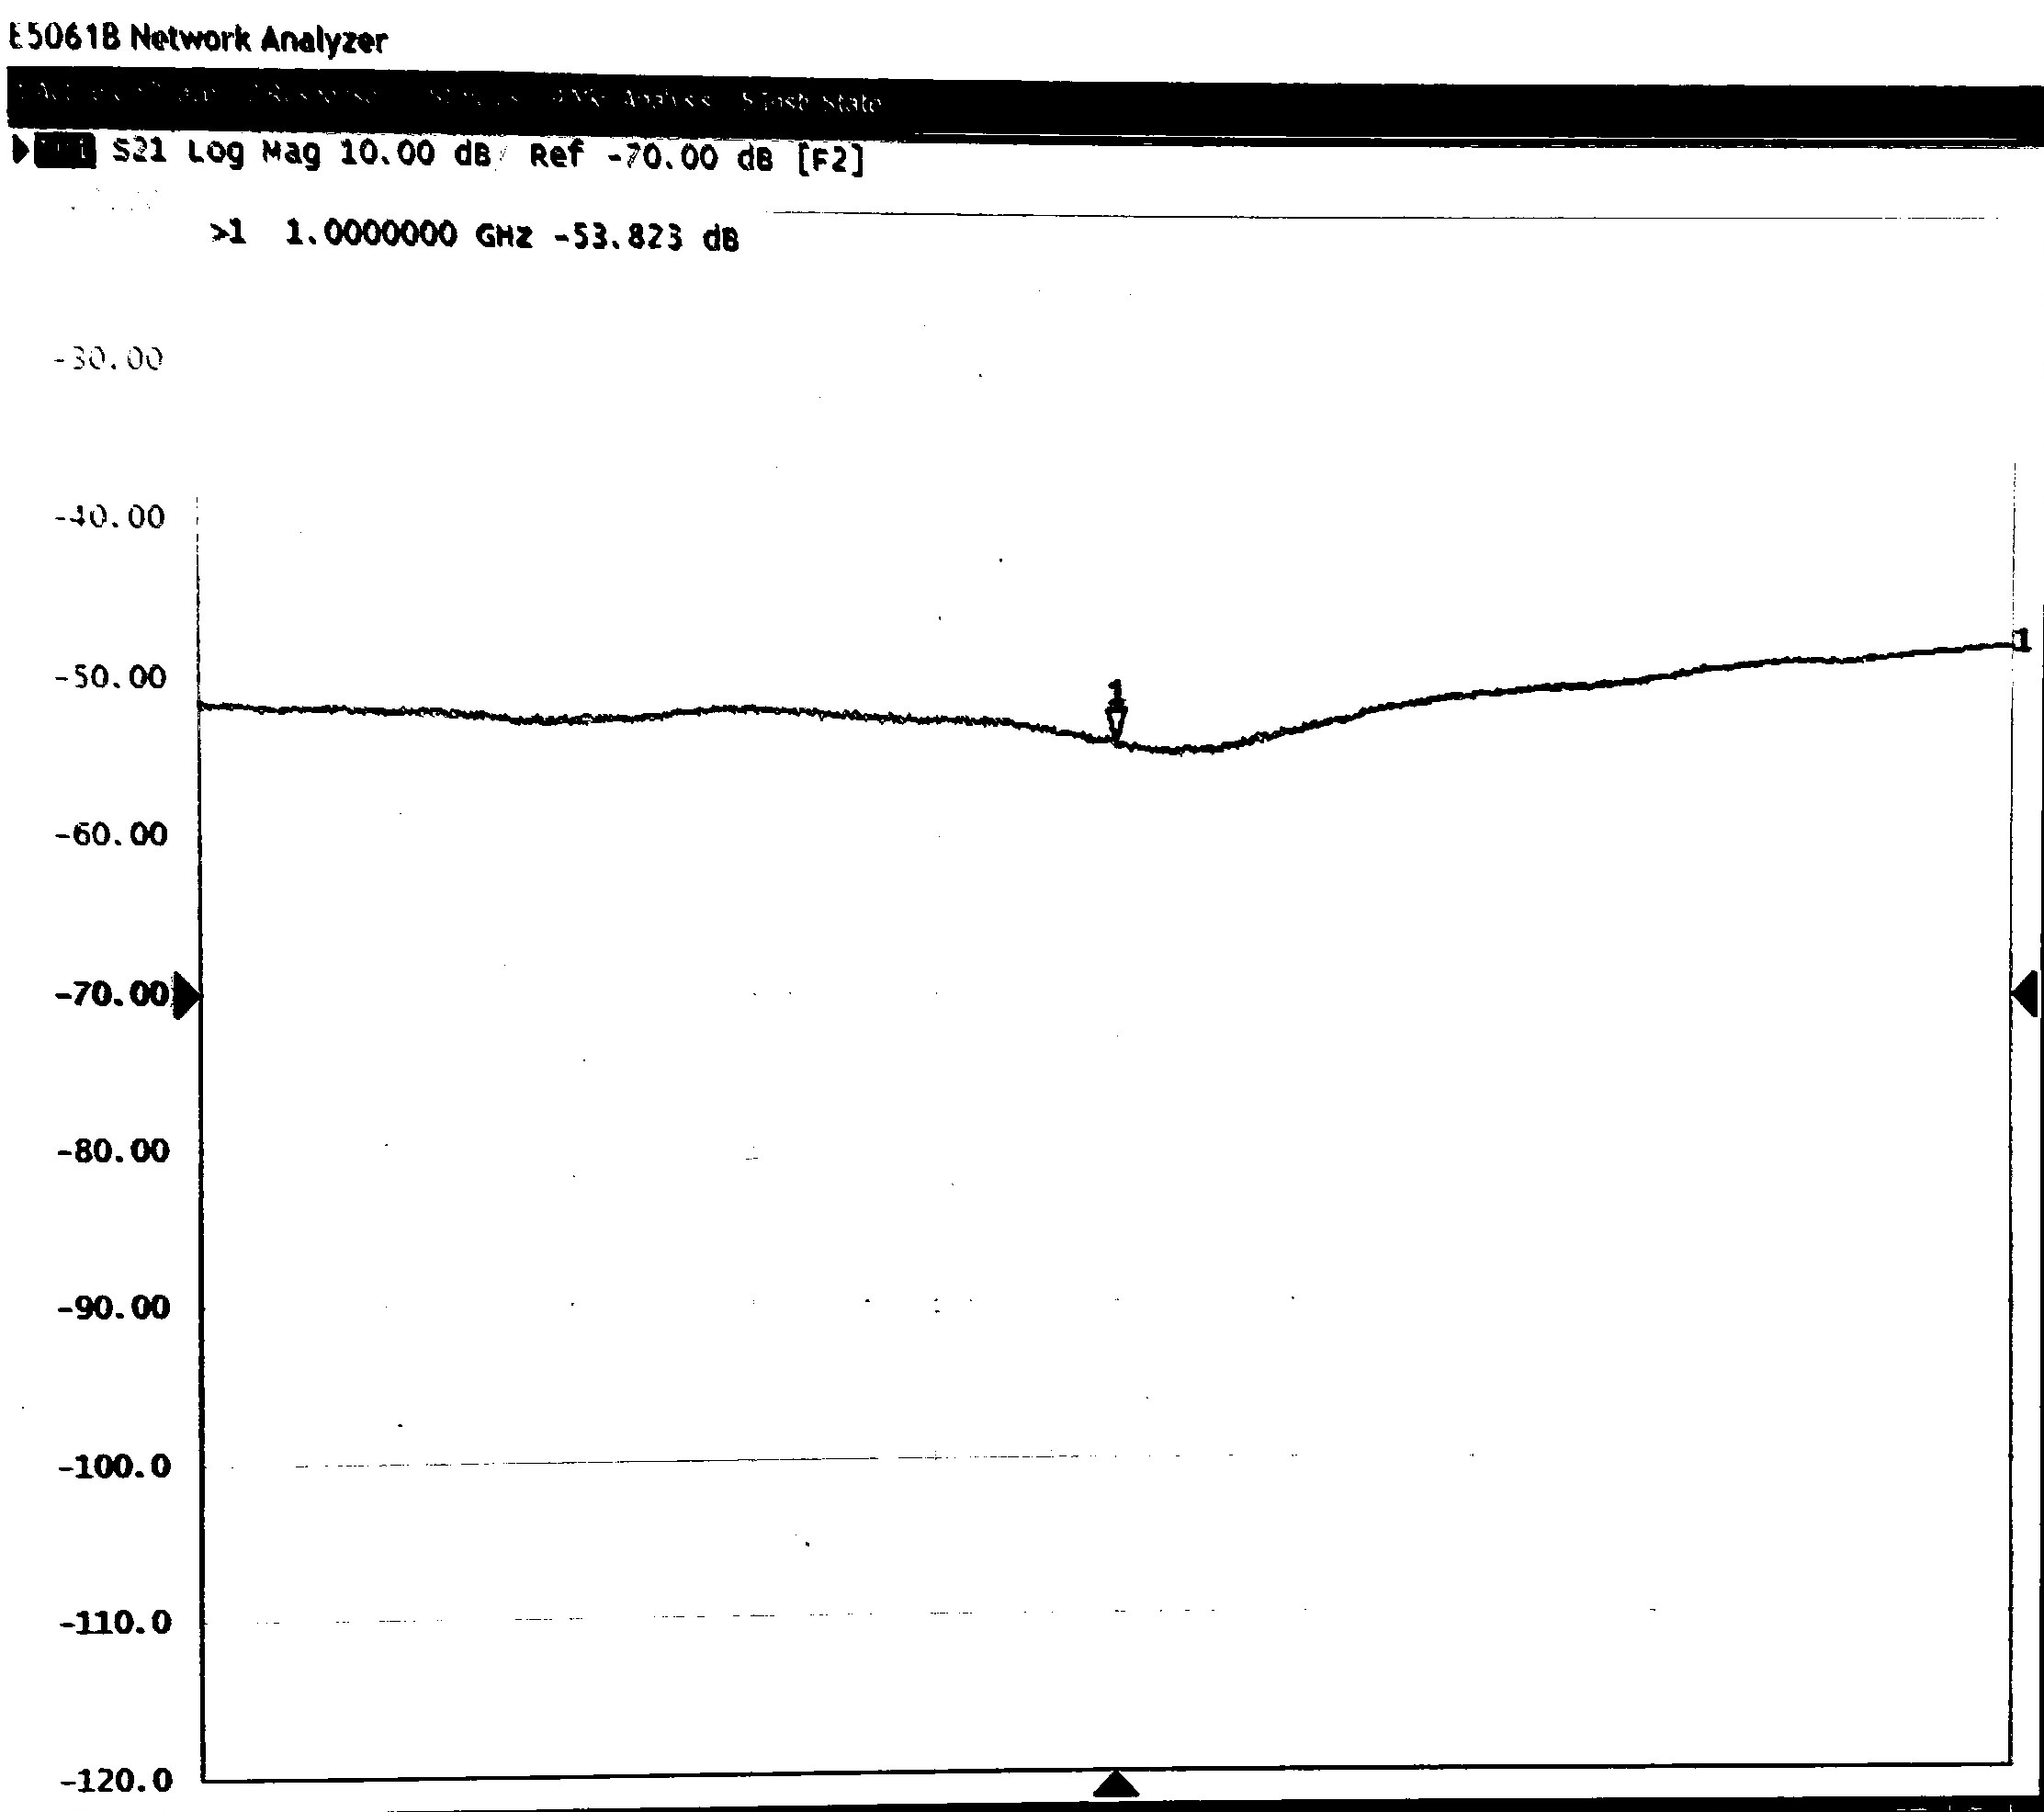
\includegraphics[width=\textwidth]{../photos/lab2/unkwn-load-valley.jpg}
      \caption{Unknown load minimum}
  \end{subfigure}
  \caption{Snapshots for measurement of maximum and minimum values of VSW pattern on the VNA}
  \label{v_t_matched_tline}
\end{figure}

\section{Notes}

All images taken during the lab were post-processed in a batch using a custom script
that bit-wise inverts the pixels and binarizes the resulting image based on a custom threshold.
No adjustments or modifications were made to the readings, for which the measurements on the VNA
are also shown alongside the waveforms. All scripts and related work can be found at 
\href{https://github.com/pranshumalik14/ece320-labs}{\texttt{github.com/pranshumalik14/ece320-labs}}.

\end{document}